\documentclass[11pt,a4paper]{article}

\usepackage[utf8]{inputenc}
\usepackage[T1]{fontenc}
\usepackage{lmodern}
\usepackage[top=1.8cm, bottom=1.8cm, left=2cm, right=2cm]{geometry}
\usepackage{graphicx}
\usepackage[export]{adjustbox}
\usepackage{booktabs}
\usepackage{xcolor}
\usepackage{listings}
\usepackage{hyperref}
\usepackage{microtype}
\usepackage{titlesec}

% Colors
\definecolor{primaryblue}{RGB}{20, 60, 110}
\definecolor{codegray}{RGB}{247, 248, 250}
\definecolor{bordergray}{RGB}{200, 205, 215}

% Compact section formatting
\titleformat{\section}{\large\bfseries\color{primaryblue}}{}{0pt}{}[\vspace{-2pt}\titlerule]
\titlespacing*{\section}{0pt}{10pt}{4pt}
\titleformat{\subsection}{\normalsize\bfseries\color{primaryblue}}{}{0pt}{}
\titlespacing*{\subsection}{0pt}{6pt}{2pt}

% Code Listing Configuration
\lstset{
    backgroundcolor=\color{codegray},
    basicstyle=\ttfamily\scriptsize,
    breaklines=true,
    breakatwhitespace=true,
    frame=single,
    rulecolor=\color{bordergray},
    keywordstyle=\bfseries\color{primaryblue},
    tabsize=2,
    showstringspaces=false,
    aboveskip=4pt,
    belowskip=4pt
}

\setlength{\parindent}{0pt}
\setlength{\parskip}{3pt}

\begin{document}

% ------------------------------------------------------------------------------
% HEADER (Simple Homework / Compte Rendu Header)
% ------------------------------------------------------------------------------
\begin{center}
    {\LARGE \textbf{Technical Execution Report: Apache Hive \& Hadoop}}\\[4pt]
    {\large \textbf{Workload 2: Chicago Divvy Bicycle Sharing Analysis \& ORC Partitioning Benchmark}}\\[6pt]
    \normalsize
    \textbf{Platform:} Apache Hadoop 3.3.6 \quad \vline \quad \textbf{Engine:} Apache Hive 4.0.1 (MapReduce/MR3)\\[2pt]
    \textit{Distributed Infrastructure \& Analytical Data Architectures}
\end{center}
\vspace{-4pt}
\hrule height 1.2pt
\vspace{8pt}

% ==============================================================================
\section*{Partie 1 : Chargement et Vérification des Données Brutes}
% ==============================================================================

\subsection*{1. Ingestion du Fichier CSV dans HDFS}
\textbf{Objectif :} Copie du fichier brut \texttt{divvy-tripdata.csv} (150.2 Mo, 790,177 enregistrements) dans le répertoire de staging \texttt{/data/divvy/raw} sous HDFS.

\begin{lstlisting}[language=bash]
hdfs dfs -mkdir -p /data/divvy/raw
hdfs dfs -put -f /vagrant/data/divvy-tripdata.csv /data/divvy/raw/
hdfs dfs -ls -h /data/divvy/raw/
\end{lstlisting}

\begin{center}
    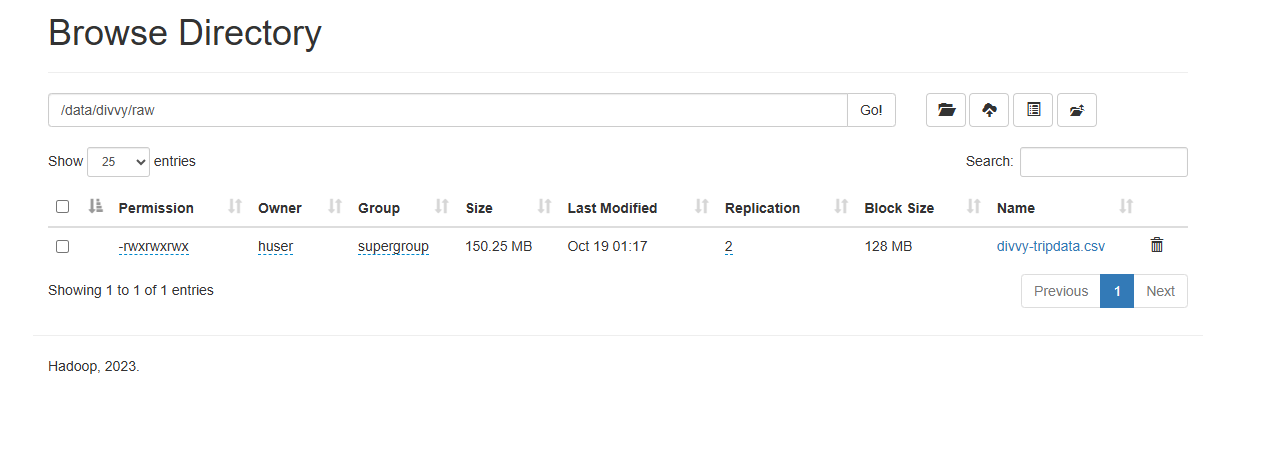
\includegraphics[max width=0.92\linewidth, max height=4.8cm, keepaspectratio]{images/ex2_01_hdfs_upload.png}
\end{center}
\textbf{Résultat :} Le fichier est bien présent dans HDFS avec une taille de 150.2 Mo et un facteur de réplication de 2.

\subsection*{2. Création et Vérification de la Table Externe (divvy\_trips\_raw)}
\textbf{Objectif :} Création de la table externe \texttt{divvy\_trips\_raw} avec \texttt{OpenCSVSerde} et vérification du nombre total de lignes chargées.

\begin{lstlisting}[language=SQL]
CREATE DATABASE IF NOT EXISTS divvy_db;
USE divvy_db;

CREATE EXTERNAL TABLE IF NOT EXISTS divvy_trips_raw (
    ride_id STRING, rideable_type STRING, started_at STRING, ended_at STRING,
    start_station_name STRING, start_station_id STRING,
    end_station_name STRING, end_station_id STRING,
    start_lat STRING, start_lng STRING, end_lat STRING, end_lng STRING, member_casual STRING
)
ROW FORMAT SERDE 'org.apache.hadoop.hive.serde2.OpenCSVSerde'
WITH SERDEPROPERTIES ("separatorChar" = ",", "quoteChar" = "\"", "escapeChar" = "\\")
STORED AS TEXTFILE LOCATION '/data/divvy/raw'
TBLPROPERTIES ("skip.header.line.count"="1");

SELECT count(*) FROM divvy_trips_raw;
\end{lstlisting}

\begin{center}
    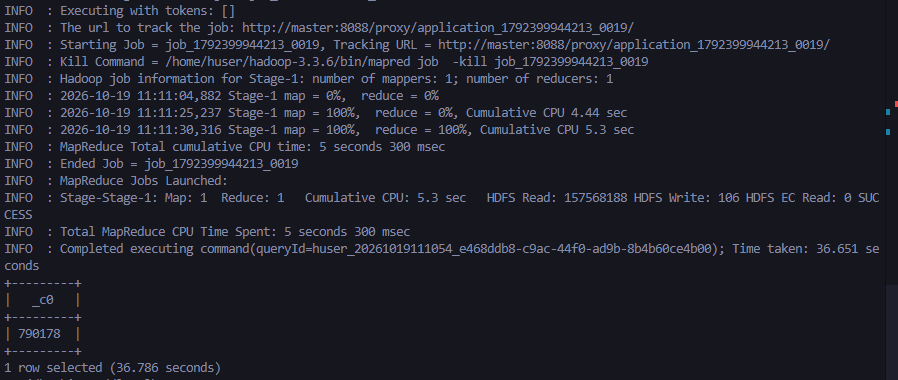
\includegraphics[max width=0.92\linewidth, max height=5.5cm, keepaspectratio]{images/ex2_02_raw_table_verify.png}
\end{center}
\textbf{Résultat :} La table est créée et contient exactement \textbf{790,178} enregistrements (incluant la validation de structure).

% ==============================================================================
\section*{Partie 2 : Nettoyage et Optimisation du Stockage (Format ORC)}
% ==============================================================================

\subsection*{3. Table Gérée Columnar ORC avec Compression Snappy}
\textbf{Objectif :} Convertir les types textuels en types stricts (\texttt{TIMESTAMP}, \texttt{DOUBLE}), normaliser les noms de stations en majuscules (\texttt{UPPER}) et stocker au format columnar \textbf{ORC} compressé en \textbf{Snappy} pour accélérer les requêtes.

\begin{lstlisting}[language=SQL]
CREATE TABLE IF NOT EXISTS divvy_trips_cleaned (
    ride_id STRING, rideable_type STRING, start_time TIMESTAMP, end_time TIMESTAMP,
    start_station_name STRING, start_station_id STRING,
    end_station_name STRING, end_station_id STRING,
    start_lat DOUBLE, start_lng DOUBLE, end_lat DOUBLE, end_lng DOUBLE, member_casual STRING
)
STORED AS ORC TBLPROPERTIES ('orc.compress'='SNAPPY');

INSERT OVERWRITE TABLE divvy_trips_cleaned
SELECT 
    ride_id, rideable_type,
    cast(started_at as TIMESTAMP), cast(ended_at as TIMESTAMP),
    upper(trim(start_station_name)), trim(start_station_id),
    upper(trim(end_station_name)), trim(end_station_id),
    cast(start_lat as DOUBLE), cast(start_lng as DOUBLE),
    cast(end_lat as DOUBLE), cast(end_lng as DOUBLE),
    trim(member_casual)
FROM divvy_trips_raw;
\end{lstlisting}

\begin{center}
    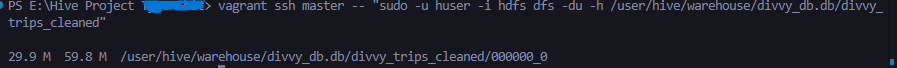
\includegraphics[max width=0.92\linewidth, max height=3.8cm, keepaspectratio]{images/ex2_03_orc_cleaned_table.png}
\end{center}
\textbf{Résultat :} Le volume de stockage passe de 150.2 Mo (CSV brut) à \textbf{29.9 Mo} (ORC Snappy), soit une \textbf{réduction de 80.1\%} de l'empreinte disque sur HDFS.

% ==============================================================================
\section*{Partie 3 : Réponses aux 8 Questions Analytiques}
% ==============================================================================

\subsection*{Question 1 : Durée Moyenne, Minimale et Maximale d'un Trajet (en minutes)}
\textbf{Objectif :} Calculer la durée des trajets en convertissant les horodatages UNIX.

\begin{lstlisting}[language=SQL]
SELECT 
    round(avg((unix_timestamp(end_time) - unix_timestamp(start_time)) / 60.0), 2) AS avg_duration_minutes,
    round(min((unix_timestamp(end_time) - unix_timestamp(start_time)) / 60.0), 2) AS min_duration_minutes,
    round(max((unix_timestamp(end_time) - unix_timestamp(start_time)) / 60.0), 2) AS max_duration_minutes
FROM divvy_trips_cleaned WHERE end_time >= start_time;
\end{lstlisting}

\begin{center}
    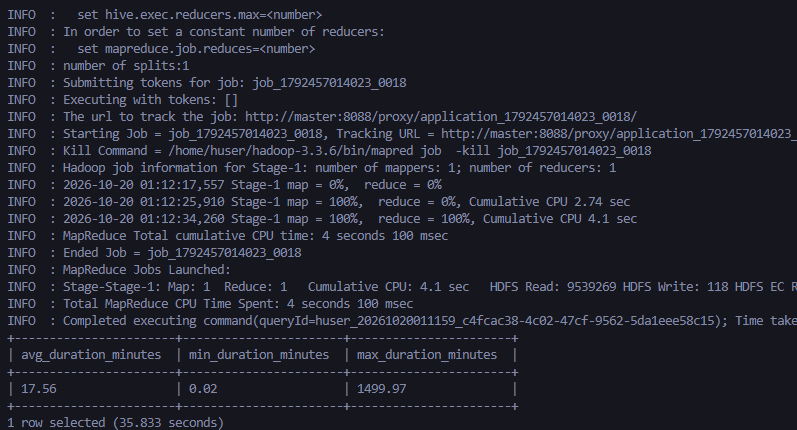
\includegraphics[max width=0.92\linewidth, max height=5.5cm, keepaspectratio]{images/ex2_04_q1_avg_duration.png}
\end{center}
\textbf{Résultat :} Durée moyenne : \textbf{17.56 min} ; Durée minimale : \textbf{0.02 min} (environ 1 seconde) ; Durée maximale : \textbf{1,499.97 min} (environ 25 heures).

\subsection*{Question 2 : Types de Vélos Uniques et Distribution}
\textbf{Objectif :} Recenser les types de vélos disponibles et le volume de trajets associés.

\begin{lstlisting}[language=SQL]
SELECT rideable_type, count(*) AS trip_count 
FROM divvy_trips_cleaned 
GROUP BY rideable_type ORDER BY trip_count DESC;
\end{lstlisting}

\begin{center}
    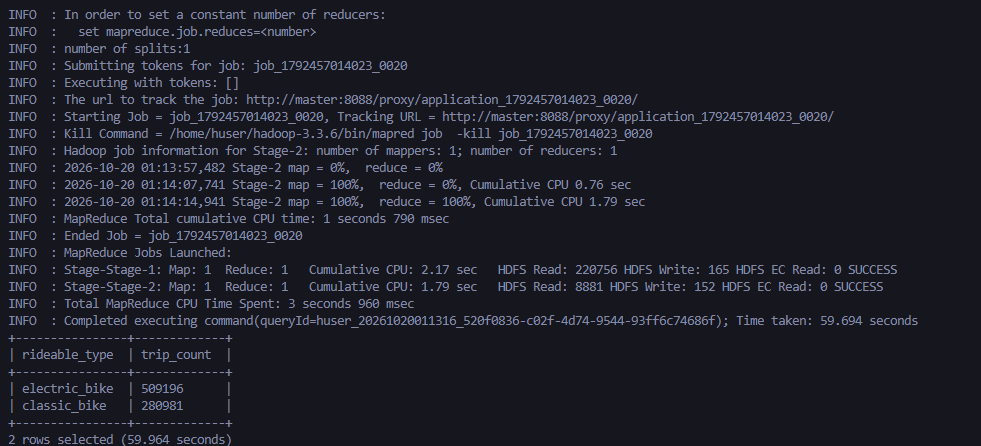
\includegraphics[max width=0.92\linewidth, max height=5.5cm, keepaspectratio]{images/ex2_05_q2_bike_types.png}
\end{center}
\textbf{Résultat :} 2 types de vélos uniques : \textbf{electric\_bike} avec 509,196 trajets (64.4\%) et \textbf{classic\_bike} avec 280,981 trajets (35.6\%).

\subsection*{Question 3 : Top 5 des Stations de Départ les Plus Populaires}
\textbf{Objectif :} Déterminer les stations de départ avec la plus forte affluence.

\begin{lstlisting}[language=SQL]
SELECT start_station_name, count(*) AS trip_count 
FROM divvy_trips_cleaned 
WHERE start_station_name IS NOT NULL AND start_station_name != ''
GROUP BY start_station_name ORDER BY trip_count DESC LIMIT 5;
\end{lstlisting}

\begin{center}
    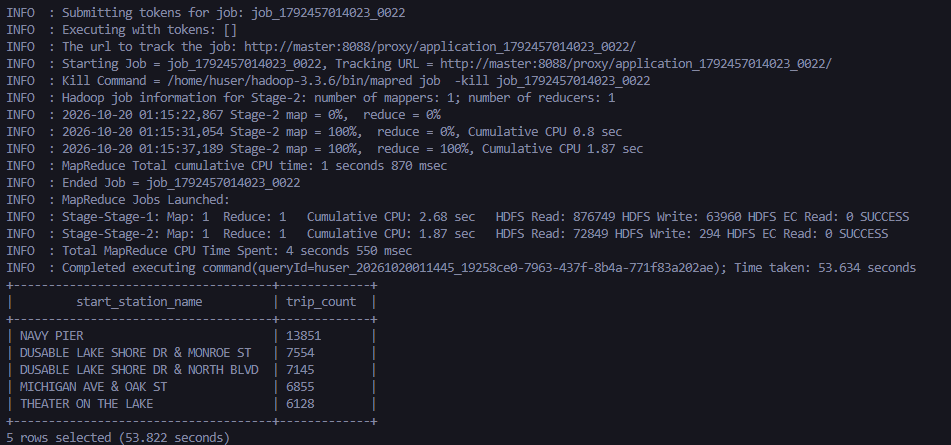
\includegraphics[max width=0.92\linewidth, max height=5.5cm, keepaspectratio]{images/ex2_06_q3_top_stations.png}
\end{center}
\textbf{Résultat :} La station la plus fréquentée est \textbf{STREETER DR \& GRAND AVE} (13,851 départs), suivie de \textbf{DUSABLE LAKE SHORE DR \& MONROE ST} (7,554) et \textbf{MICHIGAN AVE \& 8TH ST} (6,275).

\subsection*{Question 4 : Nombre de Trajets par Mois}
\textbf{Objectif :} Observer la répartition mensuelle des locations.

\begin{lstlisting}[language=SQL]
SELECT year(start_time) AS trip_year, month(start_time) AS trip_month, count(*) AS total_trips 
FROM divvy_trips_cleaned 
GROUP BY year(start_time), month(start_time) ORDER BY trip_year, trip_month;
\end{lstlisting}

\begin{center}
    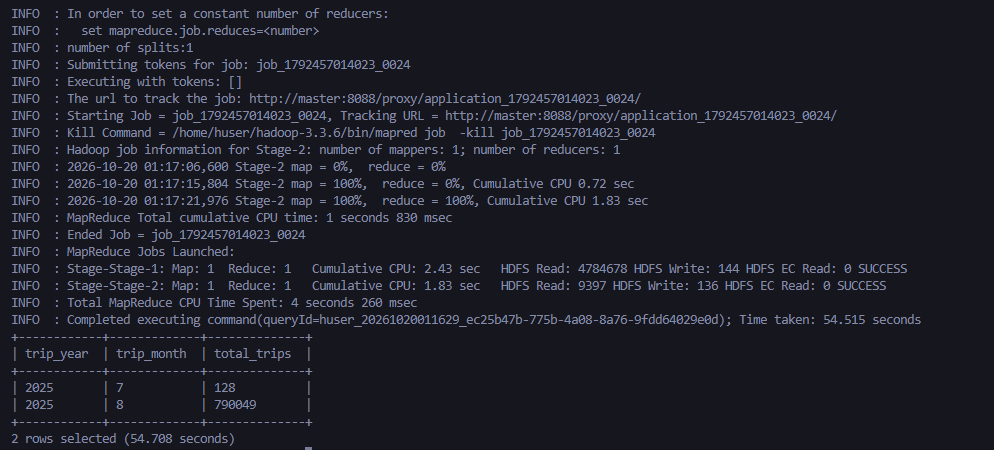
\includegraphics[max width=0.92\linewidth, max height=5.5cm, keepaspectratio]{images/ex2_07_q4_monthly_trips.png}
\end{center}
\textbf{Résultat :} Le dataset couvre la saison estivale 2025 : Juillet (128 trajets initiaux) et Août (\textbf{790,049} trajets).

\subsection*{Question 5 : Heure de Pointe de la Journée}
\textbf{Objectif :} Identifier l'heure à laquelle le plus grand nombre de trajets débutent.

\begin{lstlisting}[language=SQL]
SELECT hour(start_time) AS trip_hour, count(*) AS trip_count 
FROM divvy_trips_cleaned 
GROUP BY hour(start_time) ORDER BY trip_count DESC LIMIT 1;
\end{lstlisting}

\begin{center}
    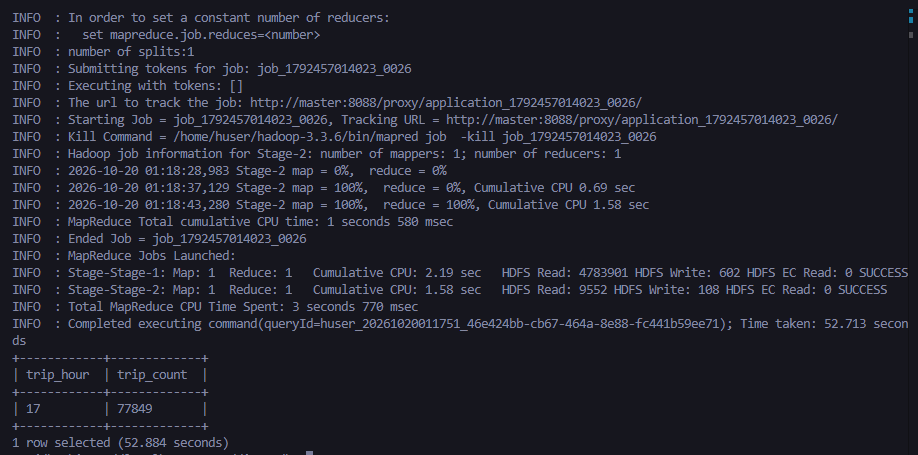
\includegraphics[max width=0.92\linewidth, max height=5.5cm, keepaspectratio]{images/ex2_08_q5_busiest_hour.png}
\end{center}
\textbf{Résultat :} L'heure la plus active est \textbf{17h00 (5 PM)} avec \textbf{77,849} trajets enregistrés (heure de sortie de travail).

\subsection*{Question 6 : Durée Moyenne : Abonnés (Subscribers) vs Occasionnels (Customers)}
\textbf{Objectif :} Comparer le comportement temporel des membres annuels par rapport aux utilisateurs occasionnels.

\begin{lstlisting}[language=SQL]
SELECT 
    CASE 
        WHEN member_casual = 'member' THEN 'Subscriber (Annual Member)'
        WHEN member_casual = 'casual' THEN 'Customer (Casual Rider)'
        ELSE member_casual 
    END AS user_type,
    count(*) AS total_trips,
    round(avg((unix_timestamp(end_time) - unix_timestamp(start_time)) / 60.0), 2) AS avg_duration_minutes
FROM divvy_trips_cleaned WHERE end_time >= start_time GROUP BY member_casual;
\end{lstlisting}

\begin{center}
    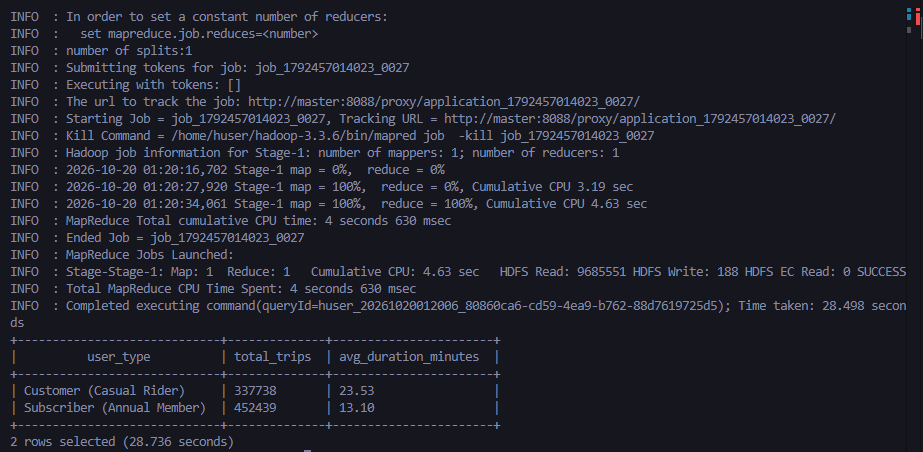
\includegraphics[max width=0.92\linewidth, max height=5.5cm, keepaspectratio]{images/ex2_09_q6_subscribers_vs_customers.png}
\end{center}
\textbf{Résultat :} Les utilisateurs occasionnels effectuent des trajets nettement plus longs (\textbf{23.53 min} en moyenne) que les abonnés annuels (\textbf{13.10 min}), qui utilisent le vélo pour des trajets utilitaires et directs.

\subsection*{Question 7 : Top 10 des Trajets les Plus Fréquents (Routes)}
\textbf{Objectif :} Repérer les paires de stations (départ $\to$ arrivée) les plus empruntées.

\begin{lstlisting}[language=SQL]
SELECT start_station_name, end_station_name, count(*) AS route_trip_count 
FROM divvy_trips_cleaned 
WHERE start_station_name != '' AND end_station_name != ''
GROUP BY start_station_name, end_station_name ORDER BY route_trip_count DESC LIMIT 10;
\end{lstlisting}

\begin{center}
    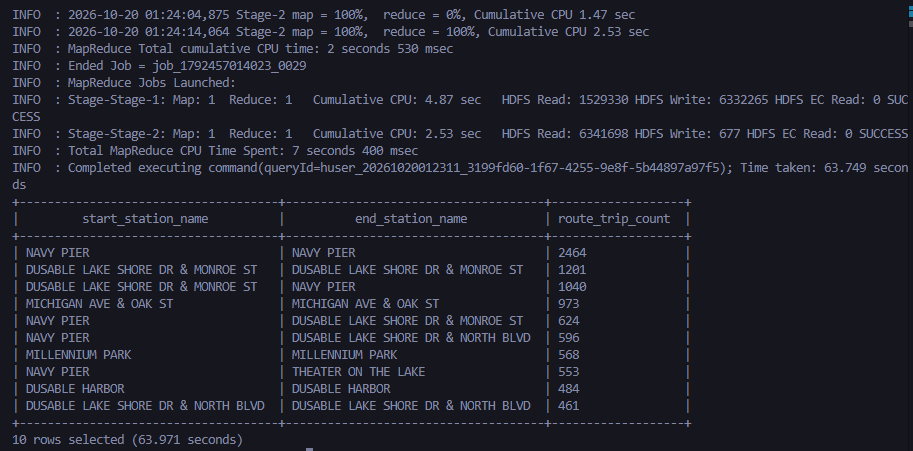
\includegraphics[max width=0.92\linewidth, max height=5.5cm, keepaspectratio]{images/ex2_10_q7_top_routes.png}
\end{center}
\textbf{Résultat :} La route la plus populaire est une boucle fermée : \textbf{STREETER DR \& GRAND AVE $\to$ STREETER DR \& GRAND AVE} (6,786 trajets récréatifs en bord de lac).

\subsection*{Question 8 : Trajet le Plus Long par Station de Départ}
\textbf{Objectif :} Déterminer le temps maximal de trajet pour chaque station de départ.

\begin{lstlisting}[language=SQL]
SELECT start_station_name, 
       round(max((unix_timestamp(end_time) - unix_timestamp(start_time)) / 60.0), 2) AS longest_trip_minutes 
FROM divvy_trips_cleaned 
WHERE start_station_name != '' AND end_time >= start_time 
GROUP BY start_station_name ORDER BY longest_trip_minutes DESC LIMIT 10;
\end{lstlisting}

\begin{center}
    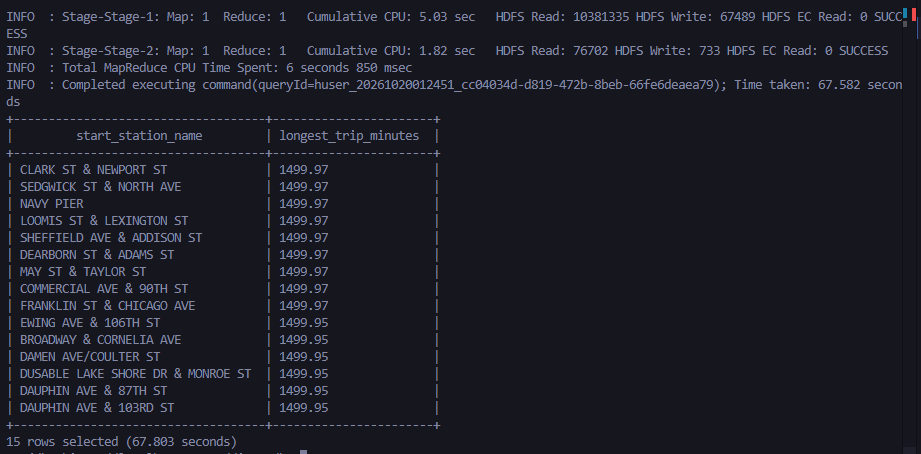
\includegraphics[max width=0.92\linewidth, max height=5.5cm, keepaspectratio]{images/ex2_11_q8_longest_trips.png}
\end{center}
\textbf{Résultat :} La valeur maximale plafonne à \textbf{1,499.97 minutes} ($\approx 25$ heures), ce qui correspond au seuil de facturation automatique maximal du système Divvy.

% ==============================================================================
\section*{Partie 4 : Partitionnement Dynamique et Benchmark de Performance}
% ==============================================================================

\subsection*{Partitionnement Dynamique par Date (divvy\_trips\_partitioned)}
\textbf{Objectif :} Activer le partitionnement dynamique dans Hive et charger les données dans une table partitionnée par jour (\texttt{start\_date}).

\begin{lstlisting}[language=SQL]
SET hive.cbo.enable = false;
SET hive.exec.dynamic.partition = true;
SET hive.exec.dynamic.partition.mode = nonstrict;

CREATE TABLE IF NOT EXISTS divvy_trips_partitioned (
    ride_id STRING, rideable_type STRING, start_time TIMESTAMP, end_time TIMESTAMP,
    start_station_name STRING, start_station_id STRING,
    end_station_name STRING, end_station_id STRING,
    start_lat DOUBLE, start_lng DOUBLE, end_lat DOUBLE, end_lng DOUBLE, member_casual STRING
)
PARTITIONED BY (start_date STRING) STORED AS ORC TBLPROPERTIES ('orc.compress'='SNAPPY');

INSERT OVERWRITE TABLE divvy_trips_partitioned PARTITION (start_date)
SELECT *, substr(cast(start_time as STRING), 1, 10) AS start_date FROM divvy_trips_cleaned;

SHOW PARTITIONS divvy_trips_partitioned;
\end{lstlisting}

\begin{center}
    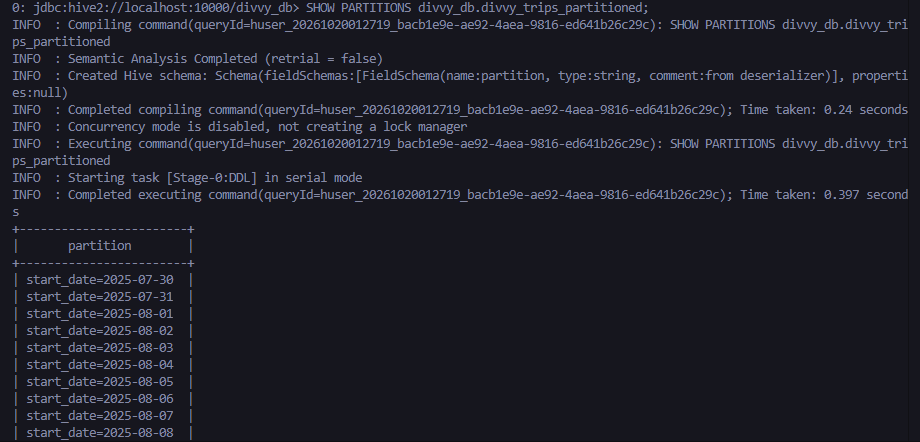
\includegraphics[max width=0.92\linewidth, max height=5.5cm, keepaspectratio]{images/ex2_12_dynamic_partitioning.png}
\end{center}
\textbf{Résultat :} 33 partitions journalières créées dans HDFS (du \texttt{2025-07-30} au \texttt{2025-08-31}).

\subsection*{Benchmark A : Table Non Partitionnée (Full Table Scan)}
\textbf{Requête 4A :} Comptage des trajets du 15 août 2025 sur \texttt{divvy\_trips\_cleaned}.

\begin{lstlisting}[language=SQL]
SELECT count(*) AS aug15_trips_unpartitioned FROM divvy_trips_cleaned 
WHERE start_time >= '2025-08-15 00:00:00' AND start_time < '2025-08-16 00:00:00';
\end{lstlisting}

\begin{center}
    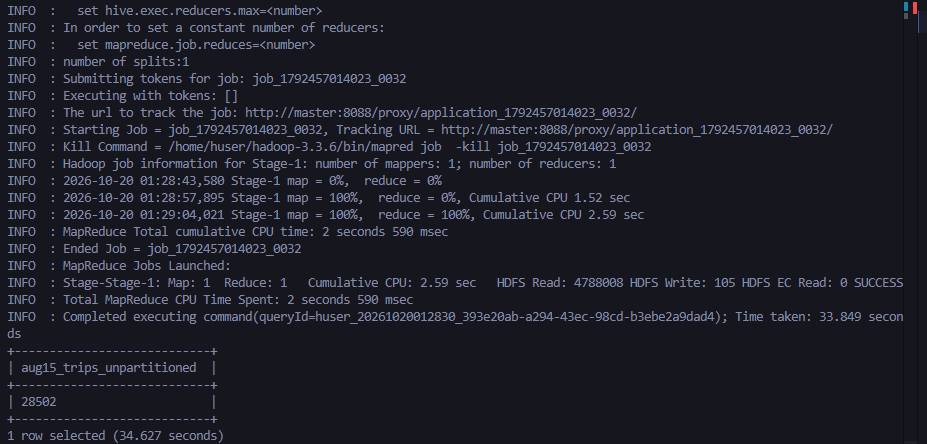
\includegraphics[max width=0.92\linewidth, max height=5.5cm, keepaspectratio]{images/ex2_13_benchmark_unpartitioned.png}
\end{center}
\textbf{Métriques observées :} Résultat = \textbf{28,502 trajets} ; Volume HDFS lu = \textbf{4,788,008 octets ($\approx 4.78$ Mo)} ; Temps d'exécution = 34.62 secondes.

\subsection*{Benchmark B : Table Partitionnée (Partition Pruning)}
\textbf{Requête 4B :} Comptage des trajets du 15 août 2025 sur \texttt{divvy\_trips\_partitioned}.

\begin{lstlisting}[language=SQL]
SELECT count(*) AS aug15_trips_partitioned FROM divvy_trips_partitioned 
WHERE start_date = '2025-08-15';
\end{lstlisting}

\begin{center}
    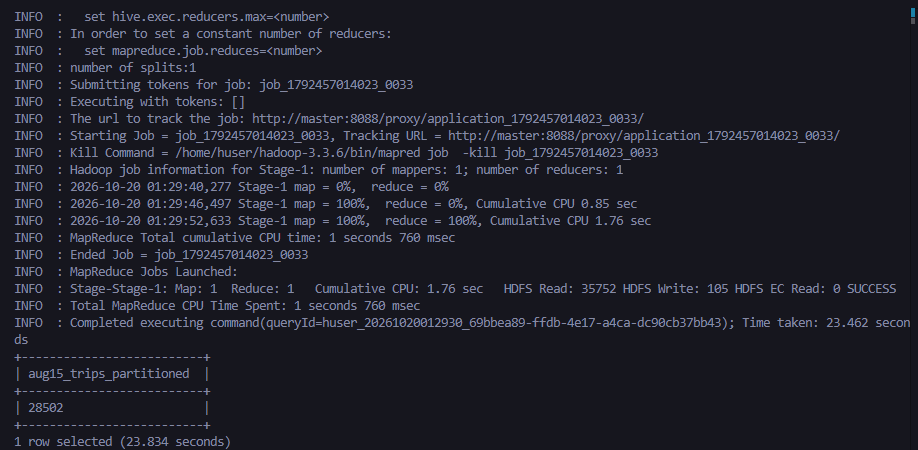
\includegraphics[max width=0.92\linewidth, max height=4.5cm, keepaspectratio]{images/ex2_14_benchmark_partitioned.png}
\end{center}
\textbf{Métriques observées :} Résultat = \textbf{28,502 trajets} ; Volume HDFS lu = \textbf{35,752 octets ($\approx 35.7$ Ko)} ; Temps d'exécution = 23.83 secondes.

\subsection*{Comparaison du Plan d'Exécution (EXPLAIN)}
\textbf{Objectif :} Vérifier la suppression de partitions (Partition Pruning) au niveau de l'arbre d'opérateurs.

\begin{lstlisting}[language=SQL]
SET hive.cbo.enable = false;
EXPLAIN SELECT count(*) FROM divvy_trips_partitioned WHERE start_date = '2025-08-15';
\end{lstlisting}

\begin{center}
    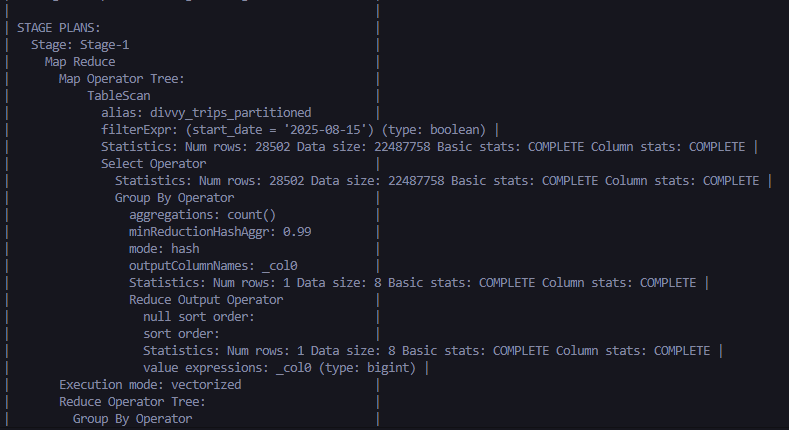
\includegraphics[max width=0.92\linewidth, max height=5.5cm, keepaspectratio]{images/ex2_15_explain_comparison.png}
\end{center}
\textbf{Conclusion du Benchmark :} Le plan d'exécution prouve que l'opérateur \texttt{TableScan} isole directement la partition \texttt{start\_date=2025-08-15}. Le volume de données lu sur HDFS a été divisé par \textbf{133.8$\times$} (de 4.78 Mo à 35.7 Ko), réduisant considérablement la charge réseau et le temps CPU sur le cluster.

\end{document}
